\documentclass[conference]{IEEEtran}
\IEEEoverridecommandlockouts
\usepackage{cite}
\usepackage{amsmath,amssymb,amsfonts}
\usepackage{array}
\usepackage{booktabs}
\usepackage{tabularx}
\usepackage{textcomp}
\usepackage{xcolor}
\usepackage{graphicx}
\usepackage{microtype}
\usepackage{url}
\def\BibTeX{{\rm B\kern-.05em{\sc i\kern-.025em b}\kern-.08em
    T\kern-.1667em\lower.7ex\hbox{E}\kern-.125emX}}

\begin{document}

\title{From Numerics to Mapping: An End-to-End Learning Pipeline\\
for Attention Accelerator Co-Design}

\author{\IEEEauthorblockN{Author Name}
\IEEEauthorblockA{\textit{Department, Institution}\\
City, Country\\
email@institution.edu}
}

\maketitle

\begin{abstract}
Long-context large language model (LLM) inference is increasingly limited by attention and key--value (KV) cache traffic rather than peak arithmetic throughput, especially during token-by-token decode.
Designing an energy-efficient attention accelerator therefore requires joint competence in FlashAttention-style numerics, mixed-precision KV compression, architecture evaluation, register-transfer-level (RTL) non-general-matrix-multiply (non-GEMM) units, and tile mapping.
This paper reports a five-project learning pipeline (P1--P5) that develops those skills on a shared LLaMA-7B-scale attention workload under a fixed hardware envelope of 128~TOPS, 1~TB/s, and 16~MiB on-chip SRAM.
P1 validates tiled and online softmax against a floating-point golden model (22/22 tests; maximum absolute error $<10^{-5}$).
P2 shows that Hadamard and block-diagonal rotation reduce INT4 key relative $\ell_2$ error by up to 41.8\% and recover KV-proxy perplexity from 3.23 to 1.93 on Qwen2.5-0.5B-Instruct.
P3 cross-checks Roofline, SCALE-Sim~v3, and Timeloop/Accelergy: decode $QK^\top$/$PV$ arithmetic intensity falls to $\approx$50.9~ops/byte (memory-bound), while weight-stationary utilization collapses from $\approx$73\% in prefill to $\approx$1\% in decode ($\approx$69$\times$).
P4 implements piecewise-linear $\exp$, online softmax reduction, and a $4\times4$ INT8 systolic array in SystemVerilog with Verilator goldens.
P5 adds a coarse FlashAttention tile simulator whose latency and traffic trends agree with SCALE-Sim on 6/6 relative checks.
We emphasize relative rather than absolute cross-tool claims and present the pipeline as scaffolding for later research stages, not as a finished accelerator.
\end{abstract}

\begin{IEEEkeywords}
Attention accelerator, FlashAttention, KV cache quantization, systolic array, SCALE-Sim, Timeloop, online softmax, software--hardware co-design.
\end{IEEEkeywords}

\section{Introduction}
\label{sec:intro}

Transformer attention~\cite{vaswani2017attention} dominates long-context LLM inference cost once prompts are long and generation proceeds autoregressively.
During \emph{prefill}, query, key, and value tensors share the prompt length and the workload is comparatively compute-friendly; during \emph{decode}, a single query row streams a growing KV cache, so bandwidth and data orchestration matter more than peak TOPS~\cite{dao2022flashattention,bitdecoding2025}.
FlashAttention reduces off-chip traffic by tiling $K$/$V$ and maintaining online softmax statistics without materializing the full score matrix~\cite{dao2022flashattention,dao2023flashattention2}.
Dedicated accelerators must still realize that dataflow under fixed SRAM and processing-element (PE) budgets, fuse non-GEMM operators that otherwise stall systolic pipelines~\cite{desa2025,lin2025systolicattention,stevens2021softermax}, and compress KV traffic with mixed precision~\cite{liu2024kivi,ashkboos2024quarot,liu2024spinquant}.

This paper does not present a new silicon design.
Instead, it documents an end-to-end \emph{learning pipeline} that builds the skills required for such co-design: numerical golden models (P1), KV quantization and rotation (P2), multi-tool architecture evaluation (P3), RTL primitives (P4), and tile-level search (P5).
The narrative is deliberately sequential: P1 supplies the golden reference used by P4; P3 supplies the bottleneck evidence and SCALE-Sim traces reused by P5; P2 motivates aggressive KV compression once P3 shows that 16~MiB can hold only about 2K INT8 tokens of $K{+}V$.

\paragraph{Contributions.}
\begin{itemize}
  \item A reproducible five-stage pipeline with shared assumptions and archival per-project reports.
  \item Quantitative evidence that decode is memory-bound and PE-starved under a conventional $32\times32$ systolic mapping, whereas prefill remains comparatively compute-bound.
  \item Empirically verified INT4+rotation error and perplexity trends, RTL bit-level checks, and tile Pareto fronts that trend-match SCALE-Sim.
\end{itemize}

\section{Background and Metrics}
\label{sec:bg}

For head dimension $d_h$, multi-head attention computes scores $S=QK^\top/\sqrt{d_h}$ and output $O=\mathrm{softmax}(S)V$~\cite{vaswani2017attention}.
FlashAttention processes $K$/$V$ in blocks while updating a running maximum $m$, an exponential sum $\ell$, and a partial output $O$ with inter-block rescaling~\cite{dao2022flashattention}.
Rotary embeddings and RMSNorm appear at the edges of the datapath in modern decoder stacks~\cite{su2024roformer,zhang2019root}.
Low-bit formats such as FP8 and INT4 reduce KV bytes but amplify outlier sensitivity; rotations (Hadamard or learned) redistribute energy before quantization~\cite{micikevicius2022fp8,ashkboos2024quarot,liu2024spinquant}.

We evaluate three layers of metrics: (i)~numerical fidelity versus a floating-point golden model; (ii)~architecture proxies---arithmetic intensity (AI), PE utilization, SRAM/DRAM traffic, and relative energy shares; and (iii)~RTL functional match to fixed-point goldens.
Across Roofline, SCALE-Sim~\cite{scalesimv3_2025}, and Timeloop/Accelergy~\cite{parashar2019timeloop,wu2019accelergy}, we compare \emph{relative} conclusions only; absolute microseconds, cycles, and joules are not equated.

\section{Method: Five-Stage Pipeline}
\label{sec:method}

\subsection{P1 --- Attention Numerics}
We implement naive scaled dot-product attention, a two-pass tiled variant, and a single-pass online-softmax kernel in PyTorch, together with RoPE, RMSNorm, and a decode-step wrapper.
Acceptance requires strict numerical agreement with library references (fp32 maximum absolute error $<10^{-5}$, block-size independence, and decode matching the last prefill token).

\subsection{P2 --- Low-Precision Quantization}
A fake-quant library covers INT4/INT8, FP8~(E4M3/E5M2), and MXFP4.
We apply random Hadamard transforms and block-diagonal Walsh--Hadamard transforms with random sign flips (BDR), following the rotation-before-quantization motif of QuaRot and SpinQuant~\cite{ashkboos2024quarot,liu2024spinquant}.
KV experiments wrap $k\_proj$/$v\_proj$ outputs on Qwen2.5-0.5B-Instruct as a \emph{proxy} for cache quantization (not token-wise cache stores).

\subsection{P3 --- Architecture Evaluation}
For a LLaMA-7B-scale layer ($d{=}4096$, $H{=}32$, $d_h{=}128$) under 128~TOPS / 1~TB/s / 16~MiB, we run Roofline AI analysis, SCALE-Sim~v3 on $32\times32$ weight- and output-stationary arrays with tiles capped at 256 per dimension, and Timeloop/Accelergy with matching tiles (45~nm PAT energy model).
The GEMMs cover $QKV$ projection, $QK^\top$, $PV$, and $O$ projection in both prefill and decode shapes.

\subsection{P4 --- RTL Building Blocks}
Three SystemVerilog modules are verified with Verilator against fixed-point or NumPy goldens: a 16-segment piecewise-linear $\exp$, an online softmax unit that maintains $m/\ell$ (without the $O$/PV accumulator), and a $4\times4$ weight-stationary INT8 systolic array.
Design notes relate rescale placement to FlashAttention-native systolic proposals such as SystolicAttention/FSA~\cite{lin2025systolicattention} and to hardware softmax co-design~\cite{stevens2021softermax}.

\subsection{P5 --- Tile-Level Simulator}
A coarse event-chain model schedules FlashAttention tiles $B_r\times B_c$ under the same 32$\times$32@1~GHz / 16~MiB / 1~TB/s envelope as P3.
Footprint legality gates feasibility; double buffering is enabled only when $2\cdot\mathrm{Footprint}\le\mathrm{SRAM}$.
Spatial MAC throughput uses $\min(B_r,R)\times\min(B_c,C)$, which exposes decode utilization collapse.
A grid search reports latency--traffic Pareto fronts and trend-checks against P3 SCALE-Sim ratios.

\section{Results}
\label{sec:results}

\subsection{P1: Golden Model Acceptance}
All 22 numerical tests pass.
Naive, tiled, and online attention agree in fp32 within $10^{-5}$ absolute error; online results are independent of block size $\{16,128\}$; RoPE and RMSNorm match Hugging Face LLaMA references; and decode-step attention matches the last prefill token.

\subsection{P2: INT4 Error and Perplexity}
Table~\ref{tab:p2} summarizes Qwen2.5-0.5B-Instruct measurements.
BDR cuts key INT4 relative $\ell_2$ by 41.8\% relative to direct quantization; both Hadamard and BDR improve end-to-end proxy perplexity relative to bare INT4.
Figure~\ref{fig:p2} shows the accompanying error-analysis plot.

\begin{table}[t]
\centering
\caption{P2 INT4 quantization on Qwen2.5-0.5B-Instruct (proxy KV via projection outputs).}
\label{tab:p2}
\begin{tabular}{@{}lrrr@{}}
\toprule
Metric & Direct & Hadamard & BDR \\
\midrule
Key rel.\ $\ell_2$ & 0.1312 & 0.0838 & 0.0763 \\
Attn-out rel.\ $\ell_2$ & 0.1207 & 0.0836 & 0.1053 \\
PPL (fp16$=$1.6840) & 3.2349 & 2.0175 & 1.9347 \\
\bottomrule
\end{tabular}
\end{table}

\begin{figure}[t]
\centering
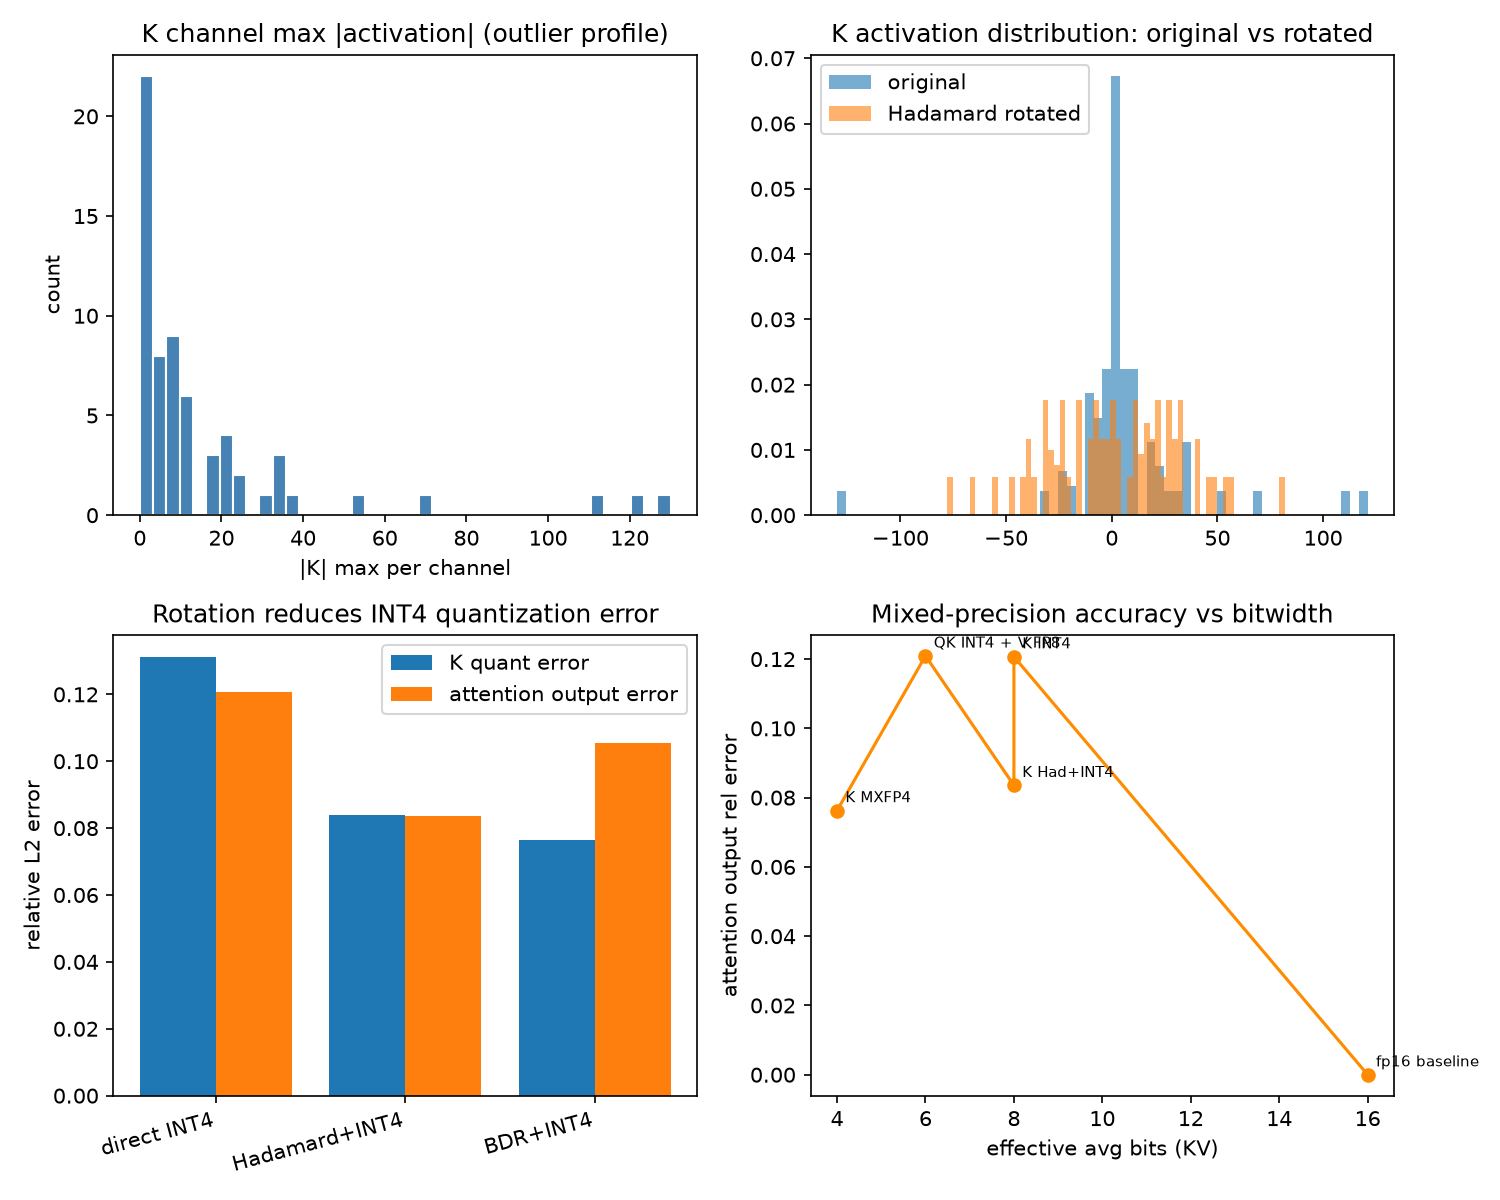
\includegraphics[width=\linewidth]{figures/error_analysis.png}
\caption{P2 fake-quant error analysis (Qwen2.5-0.5B-Instruct).}
\label{fig:p2}
\end{figure}

\subsection{P3: Decode Bottleneck Evidence}
The Roofline ridge AI is $128~\mathrm{TOPS}/1~\mathrm{TB/s}=128$~ops/byte.
At sequence length 4K, prefill $QK^\top$/$PV$ AI is $\approx$248 (compute-bound), whereas decode AI is $\approx$50.9 (memory-bound); decode projections sit near AI$\approx$2.
SCALE-Sim weight-stationary utilization for $QK^\top$/$PV$ averages $\approx$73.1\% in prefill versus $\approx$1.05\% in decode ($\approx$69$\times$ gap); output-stationary shows a $\approx$32$\times$ gap.
DRAM words account for $\approx$49\% of decode SRAM+DRAM traffic versus $\approx$37--38\% in prefill.
Timeloop PAT energy is dominated by large on-chip SRAM ($\approx$89\% decode / $\approx$99\% prefill), so we \emph{do not} claim DRAM energy dominance---only bandwidth pressure and low utilization.
Capacity math shows that 16~MiB can hold about 2048 INT8 tokens of $K{+}V$ for the full layer, which motivates tiled attention and KV compression.
Figures~\ref{fig:roofline}--\ref{fig:traffic} summarize these results.

\begin{figure}[t]
\centering
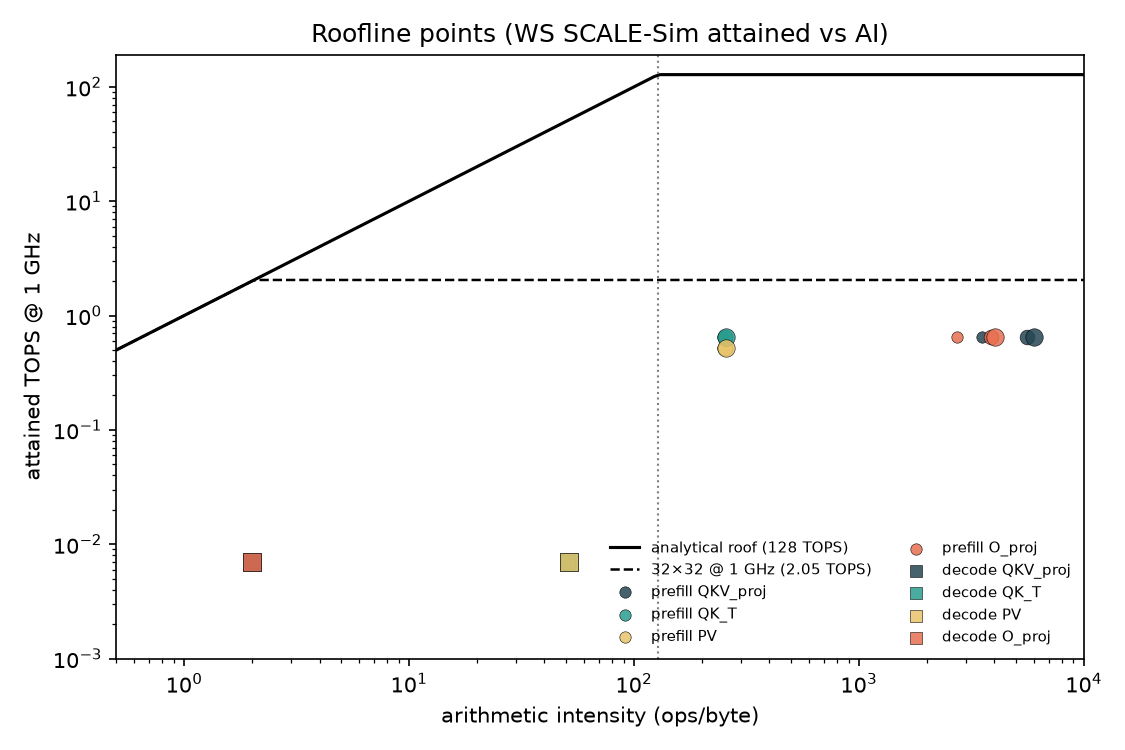
\includegraphics[width=0.95\linewidth]{figures/roofline_points.png}
\caption{P3 Roofline points (system peak 128~TOPS; array peak marked separately).}
\label{fig:roofline}
\end{figure}

\begin{figure}[t]
\centering
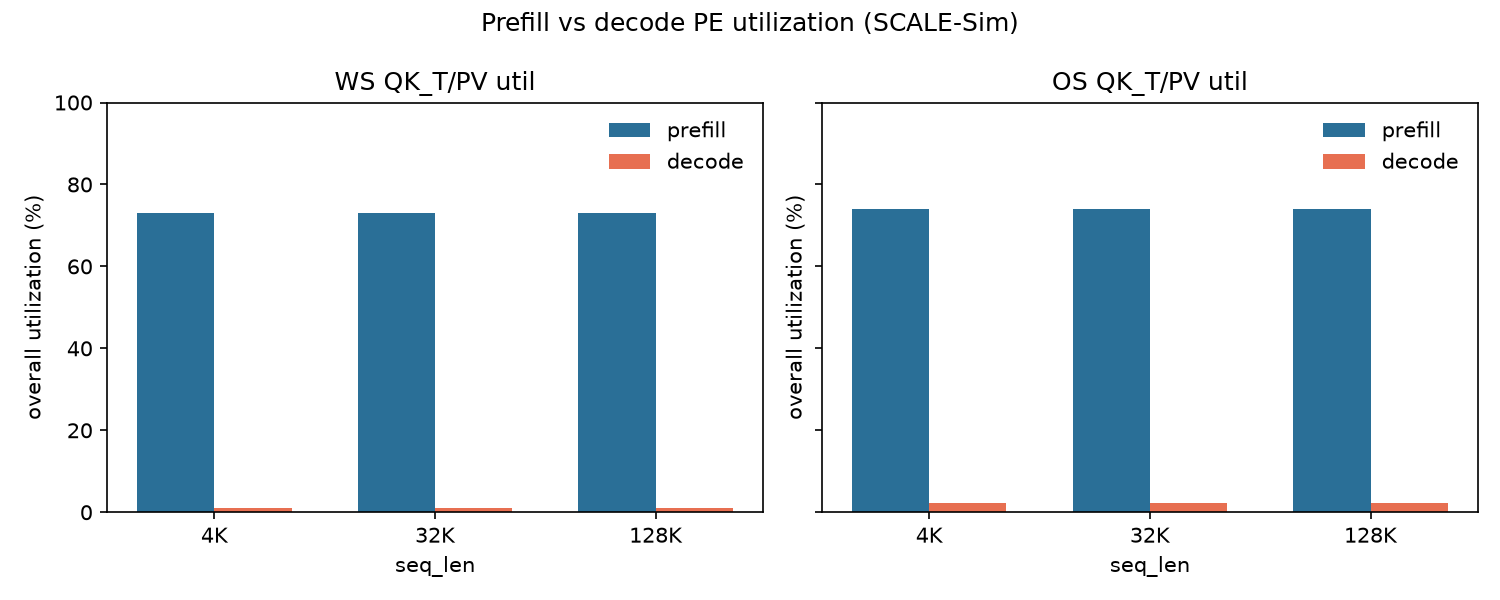
\includegraphics[width=0.95\linewidth]{figures/util_prefill_vs_decode.png}
\caption{P3 SCALE-Sim PE utilization: prefill versus decode.}
\label{fig:util}
\end{figure}

\begin{figure}[t]
\centering
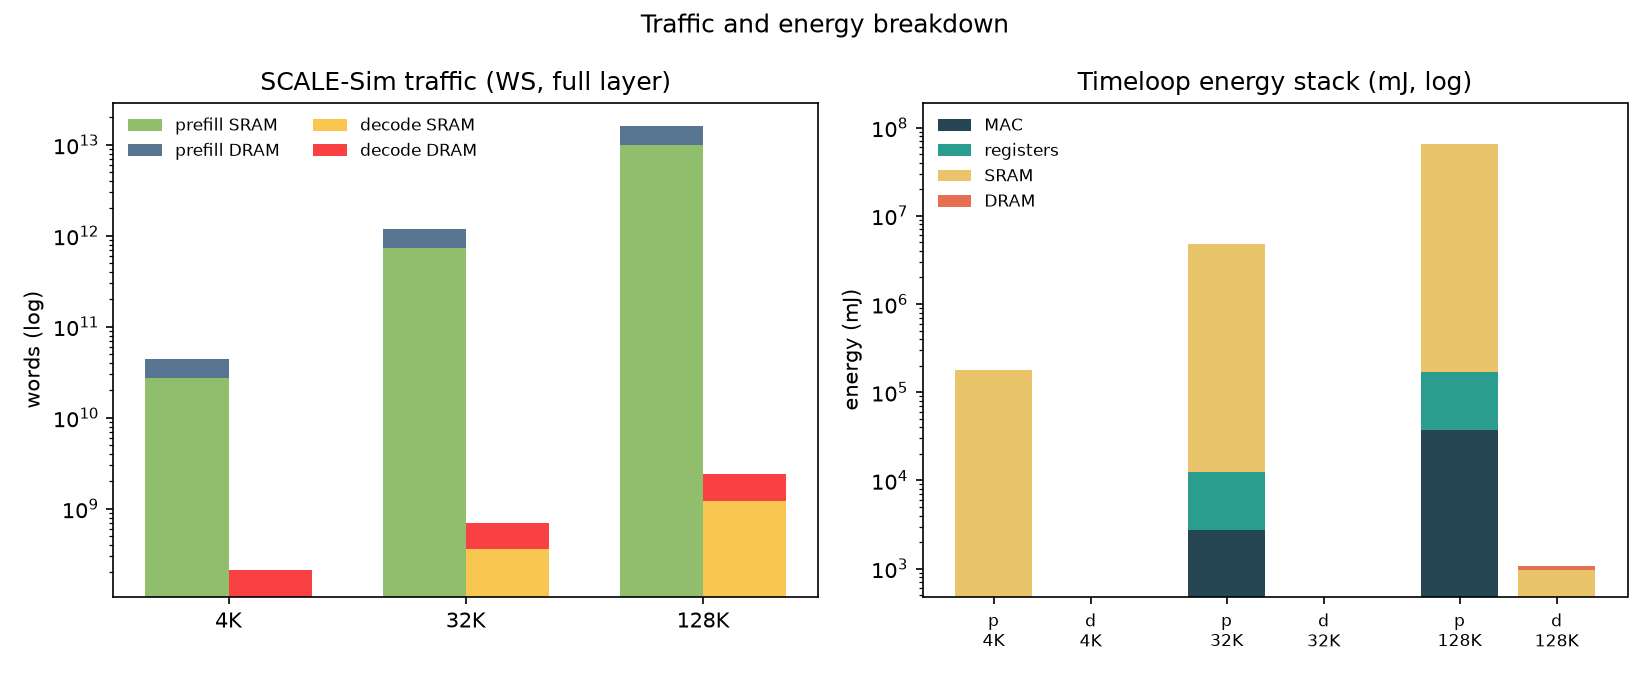
\includegraphics[width=0.95\linewidth]{figures/traffic_energy_stack.png}
\caption{P3 traffic share (left) and Timeloop energy stack (right).}
\label{fig:traffic}
\end{figure}

\subsection{P4: RTL Functional Match}
Verilator comparisons report: $\exp$---8186 samples, 0~LSB mismatch, maximum relative error $\approx3.3\times10^{-4}$ ($<10^{-3}$); online softmax---$m/\ell$ bit-exact versus the fixed-point golden; systolic array---0/32 mismatches versus NumPy INT32 GEMM for the tested matrices.

\subsection{P5: Tile Search and SCALE-Sim Trends}
At sequence length 4K, prefill Pareto search yields 81 feasible tiles (8 on the frontier); decode forces $B_r{=}1$ and collapses to a single frontier point at $B_c{=}32$ in our grid.
Cross-checks against P3 SCALE-Sim (weight-stationary, $QK^\top{+}PV$) pass 6/6 relative tests: decode utilization is much lower than prefill (SCALE-Sim $\approx$69.5$\times$, P5 $\approx$28.6$\times$, same direction); traffic and latency scale $\approx$64$\times$ (prefill) and $\approx$8$\times$ (decode) from 4K to 32K; and decode shows higher memory-pressure proxies than prefill.
Figure~\ref{fig:pareto} shows the prefill Pareto front.

\begin{figure}[t]
\centering
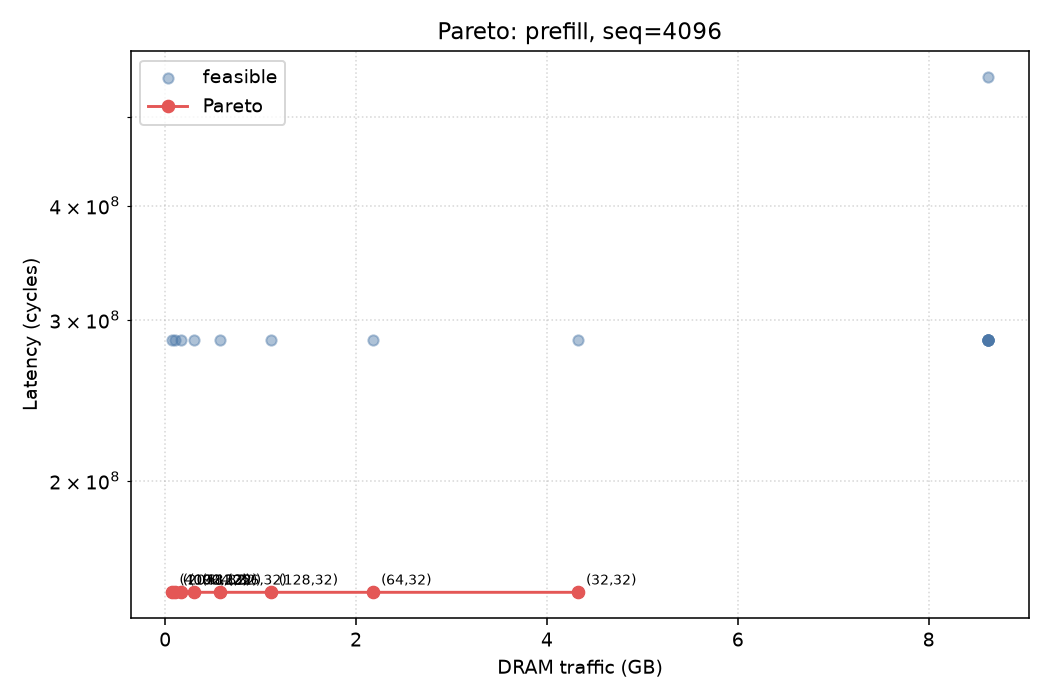
\includegraphics[width=0.95\linewidth]{figures/pareto_prefill.png}
\caption{P5 latency--traffic Pareto front (prefill, $S{=}4096$).}
\label{fig:pareto}
\end{figure}

\section{Discussion}
\label{sec:disc}

\paragraph{What the pipeline establishes.}
Taken together, P1--P5 argue that attention acceleration is a co-design problem: exact online softmax is implementable (P1/P4), KV INT4 needs outlier mitigation (P2), conventional GEMM mapping starves decode (P3/P5), and SRAM capacity forces tiling plus compression (P3).
Related accelerator and quantization literature reinforces each facet without replacing the measured trends~\cite{lin2025systolicattention,desa2025,liu2024kivi,bitdecoding2025}.

\paragraph{Limitations.}
P2 KV results are projection-output proxies on a 0.5B model.
P4 omits the $O$ accumulator and uses a toy $4\times4$ array without synthesis PPA.
P5 is not cycle-accurate and is not calibrated to P4 latencies.
Timeloop energy shares are PAT-model dependent.
These limits are acceptable for skill building but must be closed before claiming silicon-level energy per token.

\paragraph{Research mapping.}
P1 and P4 feed FlashAttention-native datapaths; P2 feeds mixed-precision stages; P3 is Stage-1 bottleneck analysis material; and P5 seeds later compile and tile-mapping work.

\section{Conclusion}
\label{sec:concl}

We presented an IEEE-style synthesis of a five-project learning pipeline for attention accelerator co-design.
The headline experimental picture is consistent across tools: decode is memory-bound and PE-starved, 16~MiB holds only a short KV tile, rotation recovers much of the INT4 perplexity penalty, and RTL and tile models can track the algorithmic intent of FlashAttention.
Future work will replace proxy quantization with true cache-path quantization, extend softmax RTL with output accumulation, and calibrate the tile simulator to measured microarchitectural latencies.

\begin{thebibliography}{00}
\bibitem{vaswani2017attention} A.~Vaswani \emph{et al.}, ``Attention is all you need,'' in \emph{NeurIPS}, 2017.
\bibitem{dao2022flashattention} T.~Dao \emph{et al.}, ``FlashAttention: Fast and memory-efficient exact attention with IO-awareness,'' in \emph{NeurIPS}, 2022.
\bibitem{dao2023flashattention2} T.~Dao, ``FlashAttention-2: Faster attention with better parallelism and work partitioning,'' arXiv:2307.08691, 2023.
\bibitem{ashkboos2024quarot} S.~Ashkboos \emph{et al.}, ``QuaRot: Outlier-free 4-bit inference in rotated LLMs,'' arXiv:2404.00456, 2024.
\bibitem{liu2024spinquant} Z.~Liu \emph{et al.}, ``SpinQuant: LLM quantization with learned rotations,'' arXiv:2405.16406, 2024.
\bibitem{liu2024kivi} Z.~Liu \emph{et al.}, ``KIVI: A tuning-free asymmetric 2bit quantization for KV cache,'' in \emph{ICML}, 2024.
\bibitem{bitdecoding2025} D.~Du \emph{et al.}, ``BitDecoding: Unlocking tensor cores for long-context LLMs with low-bit KV cache,'' arXiv:2503.18773, 2025.
\bibitem{parashar2019timeloop} A.~Parashar \emph{et al.}, ``Timeloop: A systematic approach to DNN accelerator evaluation,'' in \emph{ISPASS}, 2019.
\bibitem{wu2019accelergy} Y.~N.~Wu, J.~S.~Emer, and V.~Sze, ``Accelergy: An architecture-level energy estimation methodology for accelerator designs,'' in \emph{ICCAD}, 2019.
\bibitem{scalesimv3_2025} R.~Raj \emph{et al.}, ``SCALE-Sim v3: A modular cycle-accurate systolic accelerator simulator for end-to-end system analysis,'' arXiv:2504.15377, 2025.
\bibitem{lin2025systolicattention} J.~Lin \emph{et al.}, ``SystolicAttention: Fusing FlashAttention within a single systolic array,'' arXiv:2507.11331, 2025.
\bibitem{desa2025} Z.~Wang, H.~Fan, and G.~He, ``DESA: Dataflow efficient systolic array for acceleration of transformers,'' \emph{IEEE Trans.\ Comput.}, vol.~74, no.~6, pp.~2058--2072, 2025.
\bibitem{stevens2021softermax} J.~R.~Stevens \emph{et al.}, ``Softermax: Hardware/software co-design of an efficient softmax for transformers,'' in \emph{DAC}, 2021.
\bibitem{zhang2019root} B.~Zhang and R.~Sennrich, ``Root mean square layer normalization,'' arXiv:1910.07467, 2019.
\bibitem{su2024roformer} J.~Su \emph{et al.}, ``RoFormer: Enhanced transformer with rotary position embedding,'' \emph{Neurocomputing}, vol.~568, p.~127063, 2024.
\bibitem{micikevicius2022fp8} P.~Micikevicius \emph{et al.}, ``FP8 formats for deep learning,'' arXiv:2209.05433, 2022.
\end{thebibliography}

\end{document}
